\documentclass[11pt,a4paper]{article}
\usepackage[utf8]{inputenc}
\usepackage[T1]{fontenc}
\usepackage[french]{babel}
\usepackage[margin=2.2cm]{geometry}
\usepackage{amsmath,graphicx,booktabs,float,xcolor}
\usepackage[hidelinks]{hyperref}
\graphicspath{{resultats/}}
\hypersetup{pdfauthor={Houssam MAKHLOUK},pdftitle={TP2 - Localisation et Scan Matching}}
\begin{document}
\hypersetup{pageanchor=false}
\begin{titlepage}\centering
\vspace*{1cm}{\Large\bfseries EIGSI LA ROCHELLE\par}
\vspace{.4cm}{\large Année universitaire 2026/2027\par}
\vspace{2cm}{\large RAPPORT DE TRAVAUX PRATIQUES\par}
\vspace{.8cm}\rule{.9\textwidth}{1pt}\par\vspace{.6cm}
{\Huge\bfseries TP -- Jour 2\par}\vspace{.6cm}
{\LARGE Localisation et Scan Matching\par}\vspace{.6cm}
{\large Grille d'occupation, carte vectorielle et scans\par}
\vspace{.6cm}\rule{.9\textwidth}{1pt}
\vfill{\large Réalisé par\par}\vspace{.3cm}
{\LARGE\bfseries Houssam MAKHLOUK\par}
\vspace{.4cm}{\large Étudiant à EIGSI La Rochelle\par}
\vfill{\large 3 novembre 2026\par}
\end{titlepage}
\pagenumbering{roman}\hypersetup{pageanchor=true}
\tableofcontents\clearpage\pagenumbering{arabic}
\section{Objectif et périmètre}
Le TP demande une méthode fonctionnelle pour chacun des trois supports : grille d'occupation, carte vectorielle et scan de référence. Les trois méthodes sont comparées sur les mêmes scans et avec les mêmes poses initiales. Les erreurs de position et d'angle, les temps de calcul et la sensibilité à l'initialisation sont mesurés en simulation. Sur les données réelles, l'absence de pose terrain mesurée interdit de calculer une erreur physique indépendante.

\section{Données et séparation référence/test}
\subsection{Acquisitions réelles}
Six scans LD06 ont été enregistrés via USB/ESP32 sur COM3 à 115\,200 bauds : trois à la position A, puis trois à la position B. La hauteur annoncée à A est 1,90 m ; la même hauteur est supposée à B selon le protocole. Le déplacement effectif, l'orientation et leurs incertitudes n'ont pas été mesurés. L'absence de mouvement pendant chaque prise est une hypothèse de manipulation.
\begin{center}\begin{tabular}{lrrr}\toprule Position & Scan 1 & Scan 2 & Scan 3 \\
\midrule A & 457 & 519 & 451 \\ B & 457 & 456 & 456 \\
\bottomrule\end{tabular}\end{center}
Le nombre variable de points ne valide pas à lui seul un scan : les indices consécutifs et la couverture angulaire sont vérifiés à l'acquisition. Les données brutes restent disponibles. Les points non finis et ceux de portée hors de $[0{,}15;12]$ m sont écartés ; un point sur trois est ensuite retenu pour les essais, avec exactement le même nuage fourni aux trois solveurs.

\textbf{A\_01 seul construit toutes les références réelles.} Les scans A\_02, A\_03 et B\_01 à B\_03 sont réservés aux tests. Les points du scan de test ne sont donc pas ajoutés à la carte utilisée pour les localiser. La référence est un scan complet ; les représentations grille et vectorielle en sont dérivées.

\subsection{Simulation à poses connues}
Un environnement asymétrique est défini par un contour à décrochement et deux obstacles rectangulaires. Un raycasting de 540 directions simule des scans indépendants aux poses de référence et de test. Un bruit gaussien de distance d'écart-type 8 mm est ajouté ; les graines 11, 20 et 21 rendent les données reproductibles.
La référence est à $(0,0,0)$ ; les poses de test sont $(0{,}437;0{,}127;4{,}3^\circ)$ et $(-0{,}367;0{,}283;-6{,}4^\circ)$. Les surfaces visibles se recouvrent largement, sans être identiques : le raycasting conserve les occultations. Le décor est simple et ne représente pas toutes les difficultés d'une salle réelle.

\section{Méthodes de localisation}
La pose recherchée est $q=(x,y,\theta)$, en mètres et degrés dans les fichiers. La transformation appliquée aux points est $p_g=R(\theta)p_l+[x,y]^T$. Le signe de $Y$ des CSV est conservé.

\subsection{Sur grille d'occupation}
Une grille de 6 cm est construite depuis le scan de référence par la méthode du TP1. Pour chaque cellule, la distance au centre de la cellule occupée la plus proche est précalculée. Le score d'une pose repose sur les distances des impacts transformés aux obstacles. Un point hors carte reçoit une distance de 1 m avant plafonnement. Une cellule inconnue ne devient pas artificiellement libre ; le champ ne décrit que la distance géométrique aux obstacles connus. Ce score d'extrémités ne contrôle pas toute la cohérence des rayons traversés.

\subsection{Sur carte vectorielle}
Des segments sont extraits du scan de référence : regroupement par continuité, split-and-fit et rejet des primitives trop petites. Les seuils employés sont 35 cm pour l'écart entre voisins, 4,5 cm pour l'erreur de droite, cinq points et 15 cm de longueur minimale. Pour un segment $[a,b]$, la distance utilise la projection bornée :
\[
 t=\operatorname{clip}\left(\frac{(p-a)\cdot(b-a)}{\|b-a\|^2},0,1\right),\qquad
 d(p,[a,b])=\|p-a-t(b-a)\|.
\]
Le minimum sur les segments de la carte définit le résidu d'un point.

\subsection{Recherche multi-résolution commune aux deux cartes}
La fonction coût est $J(q)=\frac1N\sum_i\min(d(T_qp_i),0{,}6)^2$. Le plafonnement limite l'influence des points sans correspondance. Quatre niveaux explorent une grille locale en translation et orientation ; les trois meilleurs candidats sont conservés pour le niveau suivant.
\begin{center}\begin{tabular}{lrr}\toprule Niveau & Pas spatial (m) & Pas angulaire ($^\circ$) \\
\midrule 1 & 0,50 & 10 \\ 2 & 0,15 & 3 \\ 3 & 0,04 & 1 \\ 4 & 0,01 & 0,25 \\
\bottomrule\end{tabular}\end{center}
Chaque niveau teste $\pm2$ pas selon les trois dimensions. La plage théorique cumulée est donc $\pm1{,}40$ m et $\pm28{,}5^\circ$ autour du départ. Il s'agit d'une recherche locale hiérarchique, pas d'une localisation globale exhaustive de toute la salle. La résolution de la grille limite sa finesse effective.

\subsection{Entre scans : ICP}
L'ICP point-à-point transforme le scan courant, recherche les voisins dans le scan de référence et ajuste une transformation rigide par SVD. Les 85\,\% de correspondances les plus proches sont conservées. La pose est composée avec l'incrément estimé. Le calcul s'arrête après 70 itérations au maximum, ou lorsque l'incrément est inférieur à $10^{-5}$ m et $10^{-4}$ degré. La convergence vers un minimum local ne garantit pas une pose correcte ; les symétries et l'initialisation restent déterminantes.

\section{Protocole d'évaluation commun}
L'erreur de position est $e_p=\|\hat t-t^*\|$ ; l'erreur angulaire est $e_\theta=|\operatorname{wrap}(\hat\theta-\theta^*)|$, avec wrap dans $[-180^\circ,180^\circ[$. Une réussite exige simultanément $e_p\leq0{,}20$ m et $e_\theta\leq5^\circ$.

\begin{table}[H]\centering
\begin{tabular}{rrrr}\toprule Indice & $\Delta x$ (m) & $\Delta y$ (m) & $\Delta\theta$ ($^\circ$) \\
\midrule
0 & 0,00 & 0,00 & 0 \\
1 & 0,25 & 0,00 & 5 \\
2 & -0,25 & 0,15 & -5 \\
3 & 0,50 & -0,25 & 10 \\
4 & -0,50 & 0,30 & -10 \\
5 & 0,90 & 0,50 & 20 \\
6 & -0,90 & -0,50 & -20 \\
7 & 1,60 & -1,10 & 35 \\
8 & -2,00 & 1,40 & -45 \\
9 & 0,00 & 0,00 & 90 \\
\bottomrule\end{tabular}
\caption{Perturbations initiales. En simulation elles s'ajoutent aux poses exactes pour créer des cas contrôlés ; la vérité terrain n'est pas transmise aux solveurs. En réel, les cinq premières s'ajoutent à $(0,0,0)$.}
\end{table}
Deux scans simulés, dix initialisations et trois méthodes donnent 60 essais. Cinq scans réels, cinq initialisations et trois méthodes donnent 75 essais : \textbf{135 essais au total}. Les mêmes poses et points sont utilisés pour les trois méthodes dans chaque cas.
Le temps de localisation est mesuré avec \texttt{perf\_counter}, hors création des références. Le temps de préparation est enregistré séparément dans le CSV détaillé. Les temps publiés proviennent d'une exécution sur le PC de travail ; il ne s'agit pas d'un banc de performance indépendant.

\section{Résultats en simulation}
\begin{table}[H]\centering\small
\begin{tabular}{lrrrr}\toprule Méthode & $e_p$ moyen (m) & $e_\theta$ moyen ($^\circ$) & Temps médian (s) & Réussite \\
\midrule
Grille multi-résolution & 0,300 & 15,06 & 0,080 & 70\,\% \\
Segments multi-résolution & 0,294 & 14,97 & 0,250 & 70\,\% \\
ICP point-à-point & 0,217 & 13,11 & 0,161 & 80\,\% \\
\bottomrule\end{tabular}
\caption{Vingt essais par méthode. Les erreurs moyennes incluent tous les échecs, y compris les grandes perturbations.}
\end{table}
Les méthodes sur cartes réussissent 70\,\% des cas, l'ICP 80\,\%. Les sept initialisations proches réussissent sur ces deux scans ; les trois plus difficiles exposent les limites de la recherche et les minima locaux. La grille est la plus rapide sur ce jeu ; les segments demandent des projections sur plusieurs primitives pour chaque candidat. Ces résultats ne permettent pas de classer universellement les méthodes : ils dépendent des réglages, de l'environnement et du faible nombre de poses simulées.
\begin{figure}[H]\centering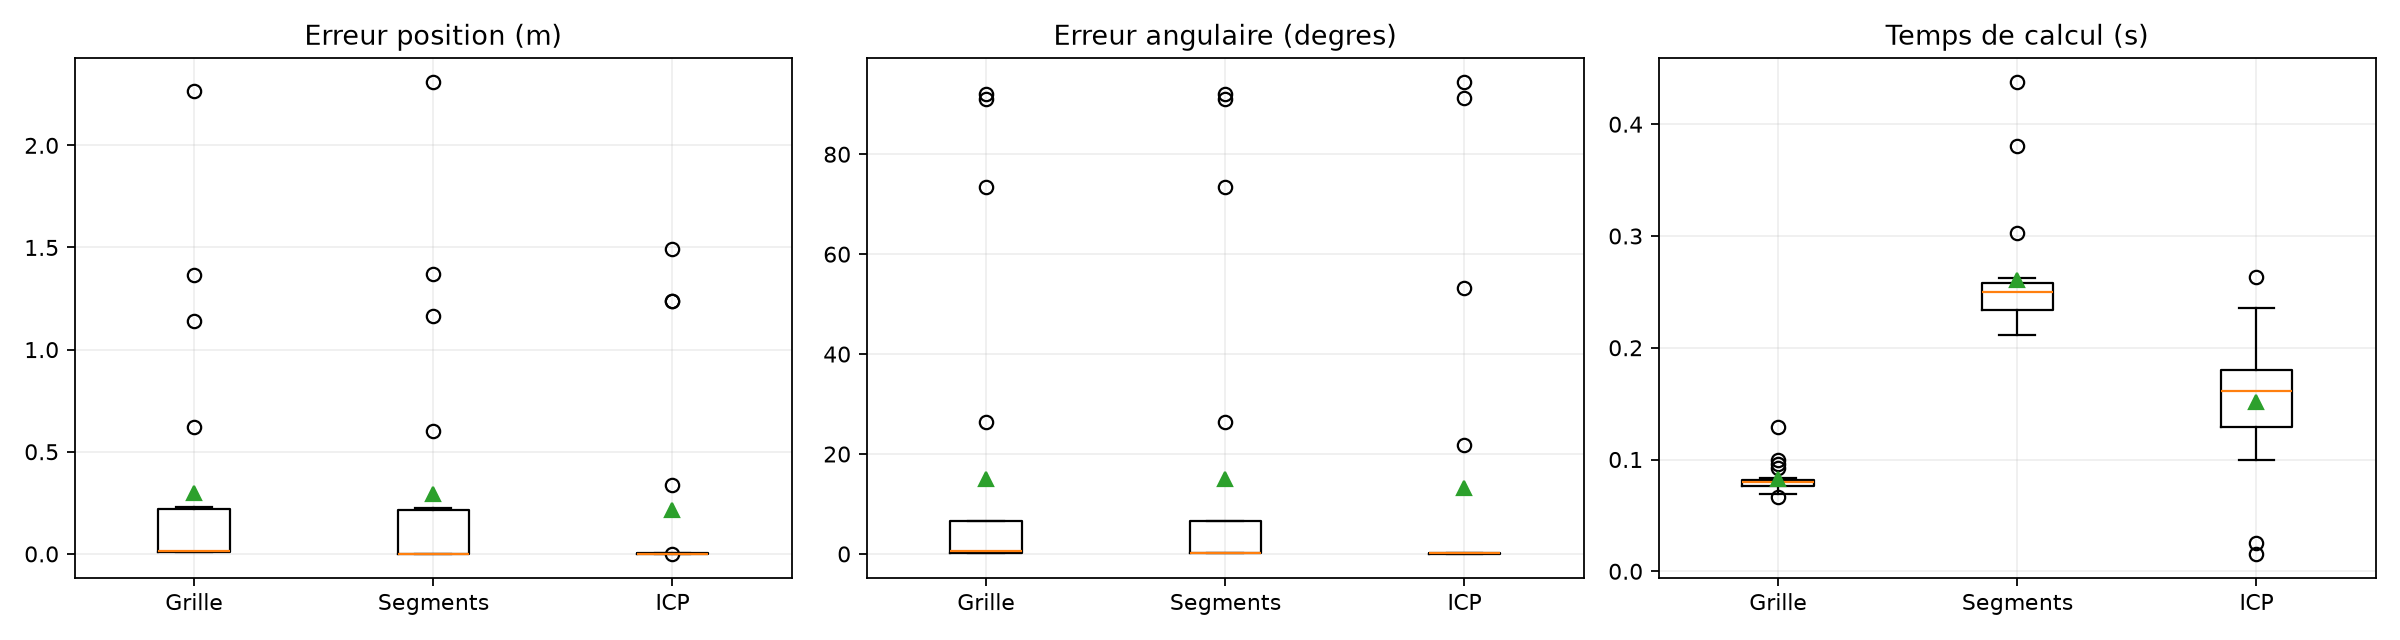
\includegraphics[width=\linewidth]{comparaison_simulation.png}\caption{Distribution des erreurs et des temps sur les essais simulés, échecs inclus.}\end{figure}
\begin{figure}[H]\centering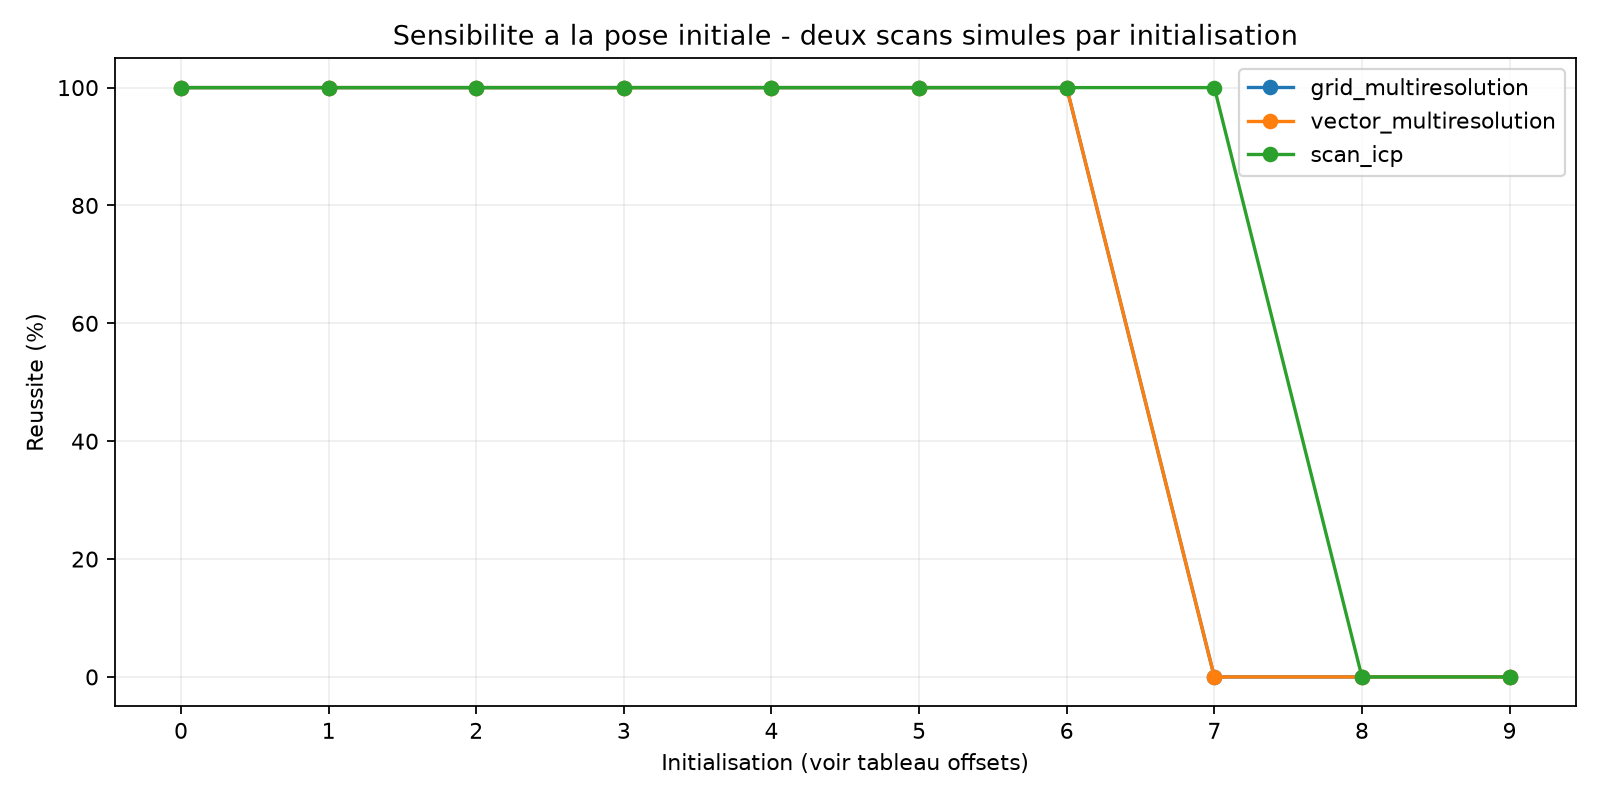
\includegraphics[width=.9\linewidth]{sensibilite_initialisation.png}\caption{Sensibilité aux dix perturbations initiales. Chaque taux par point repose seulement sur deux scans, donc varie par pas de 50\,\%.}\end{figure}
\begin{figure}[H]\centering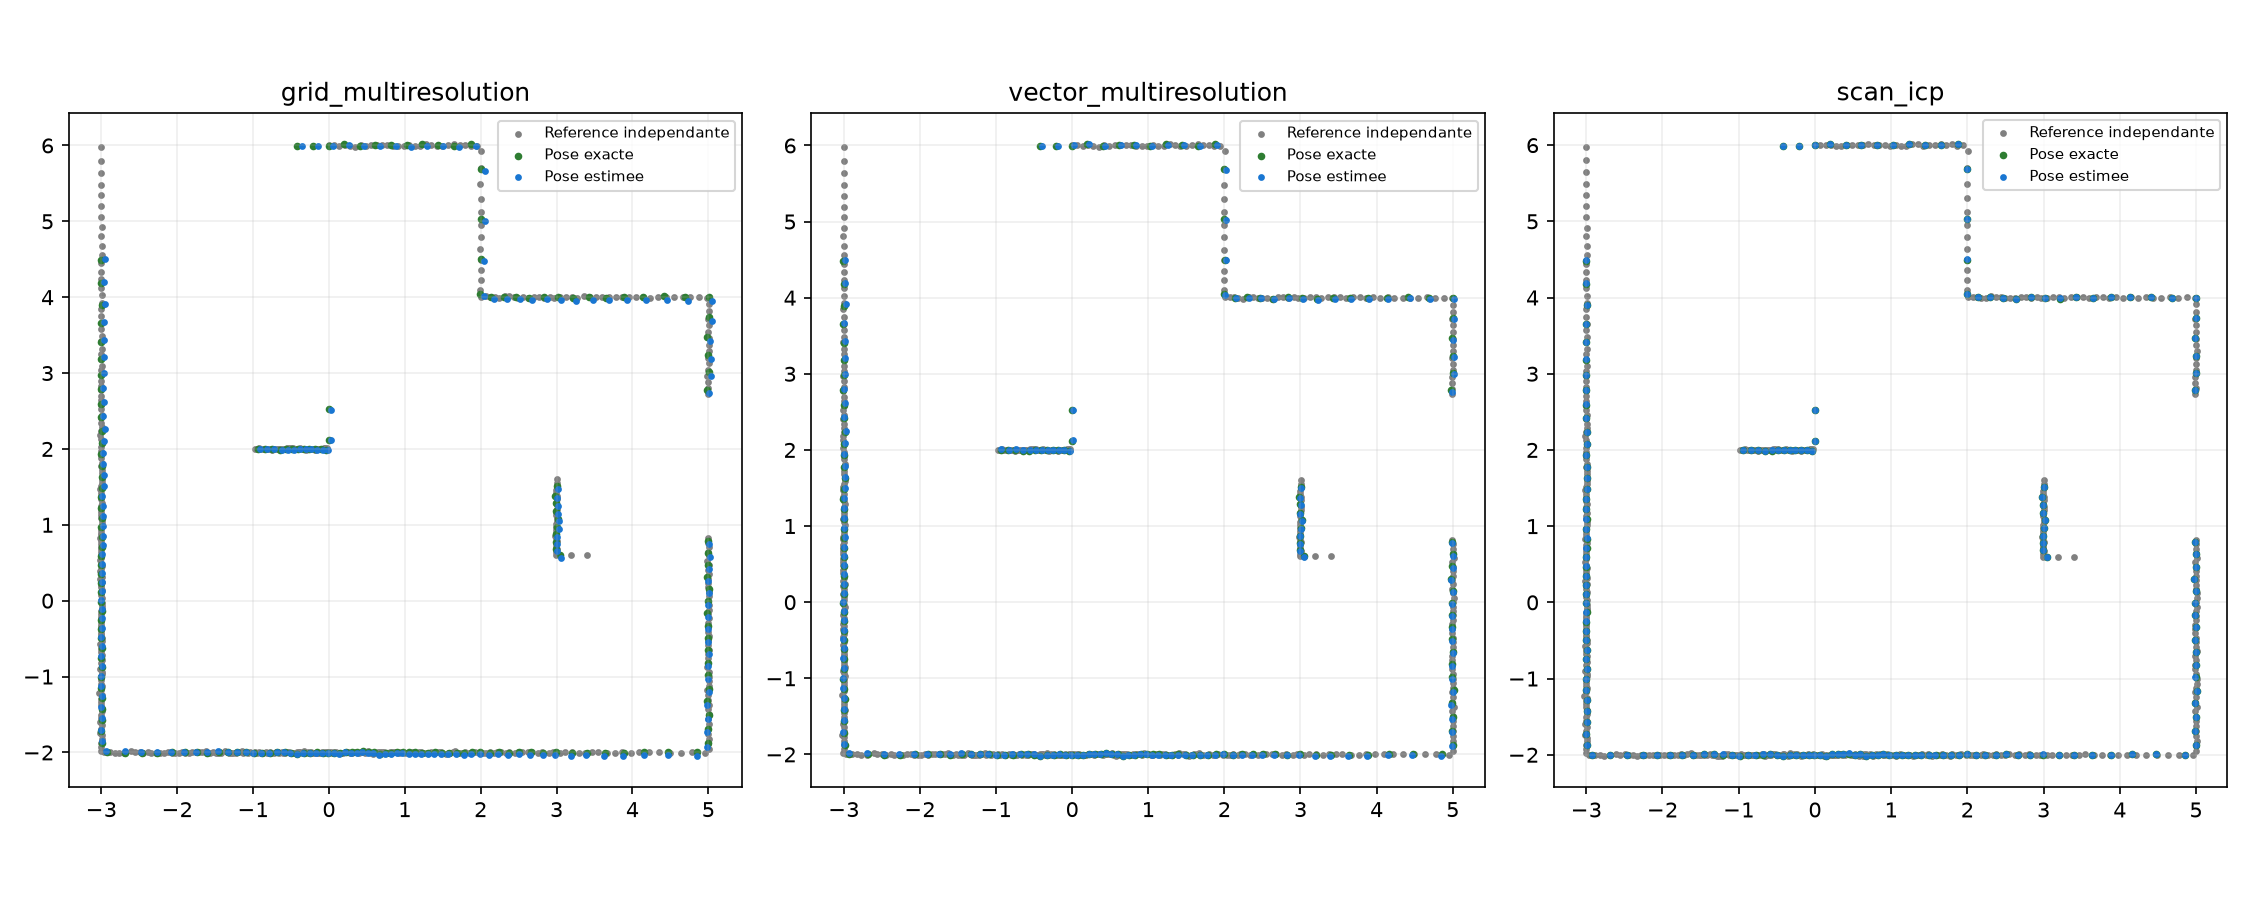
\includegraphics[width=\linewidth]{simulation_localisation.png}\caption{Exemple de localisation des trois méthodes, au départ exact pour isoler la cohérence du modèle.}\end{figure}

\section{Résultats sur les acquisitions réelles}
\begin{table}[H]\centering
\begin{tabular}{lrr}\toprule Méthode & Temps médian (s) & Résidu moyen plafonné (m) \\
\midrule
Grille multi-résolution & 0,079 & 0,050 \\
Segments multi-résolution & 0,221 & 0,033 \\
ICP point-à-point & 0,106 & 0,051 \\
\bottomrule\end{tabular}
\caption{Vingt-cinq essais réels par méthode. Les résidus utilisent des références différentes et ne doivent pas être assimilés à des erreurs de pose comparables.}\end{table}
Depuis la pose initiale $(0,0,0)$, les estimations pour B\_01 sont :
\begin{center}\small\begin{tabular}{lrrr}\toprule M?thode & $x$ (m) & $y$ (m) & $\theta$ ($^\circ$) \\
\midrule Grille & $-0{,}870$ & $-0{,}040$ & $-0{,}75$ \\
Segments & $-0{,}890$ & $-0{,}040$ & $-1{,}00$ \\
ICP & $-0{,}872$ & $-0{,}068$ & $-0{,}30$ \\
\bottomrule\end{tabular}\end{center}
Le d?placement estim? est proche de 0,9 m, et non une distance physique valid?e. Les autres scans et d?parts figurent dans le CSV complet.
\begin{figure}[H]\centering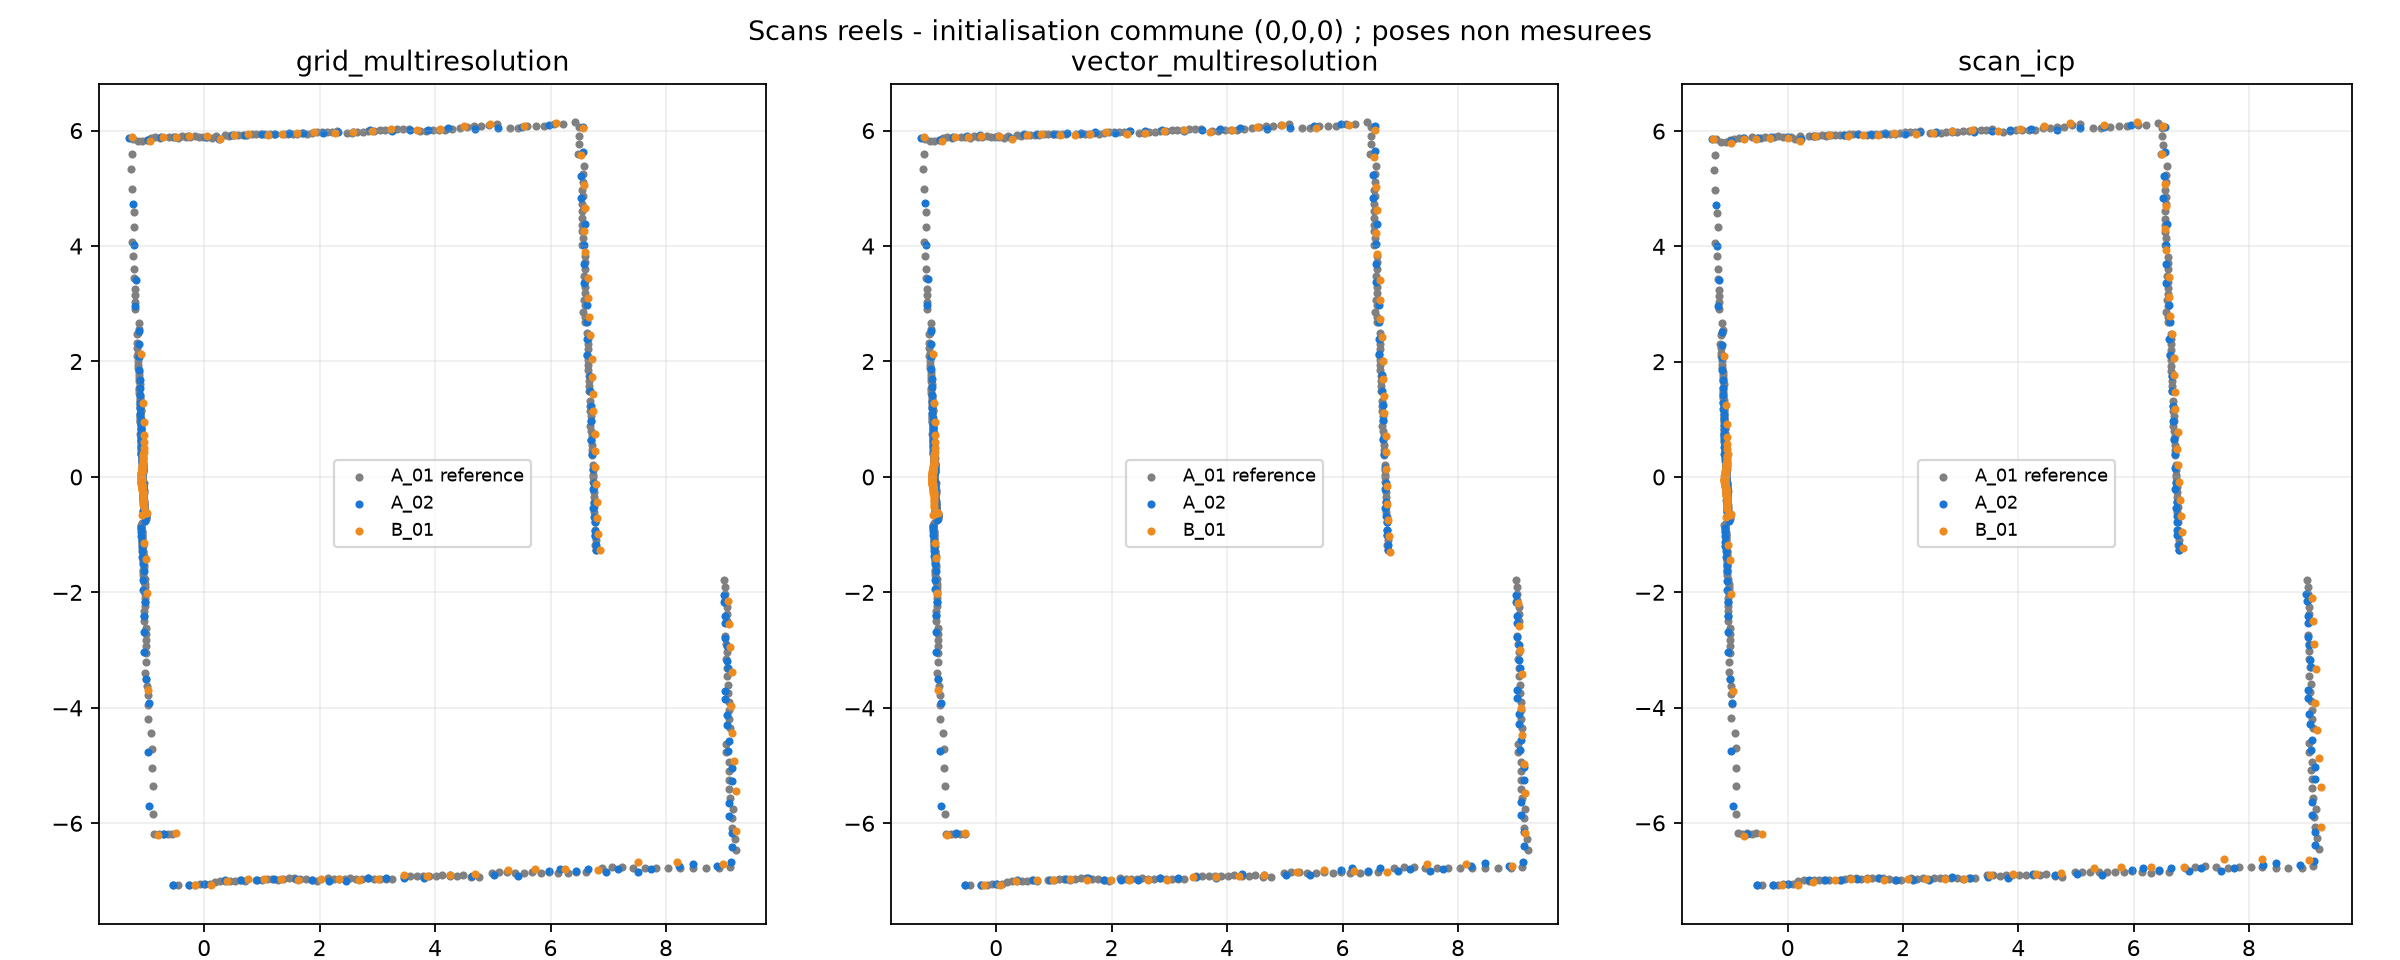
\includegraphics[width=\linewidth]{localisation_reelle.png}\caption{Référence A\_01 et scans de test A\_02/B\_01 recalés depuis la même pose initiale nulle.}\end{figure}
\textbf{Référence terrain : non mesurée. Incertitudes de position et d'angle : non disponibles.} Les erreurs métriques et les taux de réussite réels sont donc laissés non renseignés, et non remplacés par des zéros. Ni le résidu, ni l'accord de trois algorithmes, ni leur dispersion ne remplace l'incertitude d'une mesure indépendante. Pour satisfaire une évaluation métrique sur robot, il reste à relever les positions et orientations avec un moyen indépendant et à documenter sa précision.

\section{Tests, reproduction et limites}
Sept tests vérifient les angles, distances aux segments, pénalités hors carte, raycasting analytique, récupération d'une transformation connue par ICP, fonctionnement des deux solveurs sur cartes et rejet de scans invalides.
\begin{verbatim}
python tp2/evaluer.py
python -m unittest discover -s tp2 -p "test_*.py" -v
\end{verbatim}
Les exports comprennent les 135 essais détaillés, la synthèse, les paramètres, les poses simulées exactes, les grilles et les figures. Les graines sont fixes mais les temps fluctuent selon la machine. Le code dépend des modules du TP1 conservés dans \texttt{tp1/LD06\_Atelier}.
Les limites principales sont le petit jeu simulé, le sous-échantillonnage, la portée locale de la recherche, les symétries, la discrétisation de la grille, les occultations et l'absence de référence terrain réelle. Les méthodes ne réalisent pas un SLAM ni une fermeture de boucle.

\section{Conclusion}
Une méthode fonctionnelle est fournie pour chacun des trois types de référence. Le protocole compare les mêmes scans et départs et mesure les erreurs, temps et taux de réussite en simulation. Les acquisitions réelles montrent une cohérence entre méthodes mais ne permettent pas de conclure sur la précision physique sans référence indépendante. La validation quantitative sur robot reste donc à compléter si elle est exigée, avec des mesures et incertitudes documentées.
\end{document}
